\documentclass[]{article}
\usepackage{lmodern}
\usepackage{amssymb,amsmath}
\usepackage{ifxetex,ifluatex}
\usepackage{fixltx2e} % provides \textsubscript
\ifnum 0\ifxetex 1\fi\ifluatex 1\fi=0 % if pdftex
  \usepackage[T1]{fontenc}
  \usepackage[utf8]{inputenc}
\else % if luatex or xelatex
  \ifxetex
    \usepackage{mathspec}
  \else
    \usepackage{fontspec}
  \fi
  \defaultfontfeatures{Ligatures=TeX,Scale=MatchLowercase}
\fi
% use upquote if available, for straight quotes in verbatim environments
\IfFileExists{upquote.sty}{\usepackage{upquote}}{}
% use microtype if available
\IfFileExists{microtype.sty}{%
\usepackage{microtype}
\UseMicrotypeSet[protrusion]{basicmath} % disable protrusion for tt fonts
}{}
\usepackage[margin=1in]{geometry}
\usepackage{hyperref}
\hypersetup{unicode=true,
            pdftitle={Estimation of subnational fertility in SSA},
            pdfauthor={Oli Stevens},
            pdfborder={0 0 0},
            breaklinks=true}
\urlstyle{same}  % don't use monospace font for urls
\usepackage{color}
\usepackage{fancyvrb}
\newcommand{\VerbBar}{|}
\newcommand{\VERB}{\Verb[commandchars=\\\{\}]}
\DefineVerbatimEnvironment{Highlighting}{Verbatim}{commandchars=\\\{\}}
% Add ',fontsize=\small' for more characters per line
\usepackage{framed}
\definecolor{shadecolor}{RGB}{248,248,248}
\newenvironment{Shaded}{\begin{snugshade}}{\end{snugshade}}
\newcommand{\KeywordTok}[1]{\textcolor[rgb]{0.13,0.29,0.53}{\textbf{#1}}}
\newcommand{\DataTypeTok}[1]{\textcolor[rgb]{0.13,0.29,0.53}{#1}}
\newcommand{\DecValTok}[1]{\textcolor[rgb]{0.00,0.00,0.81}{#1}}
\newcommand{\BaseNTok}[1]{\textcolor[rgb]{0.00,0.00,0.81}{#1}}
\newcommand{\FloatTok}[1]{\textcolor[rgb]{0.00,0.00,0.81}{#1}}
\newcommand{\ConstantTok}[1]{\textcolor[rgb]{0.00,0.00,0.00}{#1}}
\newcommand{\CharTok}[1]{\textcolor[rgb]{0.31,0.60,0.02}{#1}}
\newcommand{\SpecialCharTok}[1]{\textcolor[rgb]{0.00,0.00,0.00}{#1}}
\newcommand{\StringTok}[1]{\textcolor[rgb]{0.31,0.60,0.02}{#1}}
\newcommand{\VerbatimStringTok}[1]{\textcolor[rgb]{0.31,0.60,0.02}{#1}}
\newcommand{\SpecialStringTok}[1]{\textcolor[rgb]{0.31,0.60,0.02}{#1}}
\newcommand{\ImportTok}[1]{#1}
\newcommand{\CommentTok}[1]{\textcolor[rgb]{0.56,0.35,0.01}{\textit{#1}}}
\newcommand{\DocumentationTok}[1]{\textcolor[rgb]{0.56,0.35,0.01}{\textbf{\textit{#1}}}}
\newcommand{\AnnotationTok}[1]{\textcolor[rgb]{0.56,0.35,0.01}{\textbf{\textit{#1}}}}
\newcommand{\CommentVarTok}[1]{\textcolor[rgb]{0.56,0.35,0.01}{\textbf{\textit{#1}}}}
\newcommand{\OtherTok}[1]{\textcolor[rgb]{0.56,0.35,0.01}{#1}}
\newcommand{\FunctionTok}[1]{\textcolor[rgb]{0.00,0.00,0.00}{#1}}
\newcommand{\VariableTok}[1]{\textcolor[rgb]{0.00,0.00,0.00}{#1}}
\newcommand{\ControlFlowTok}[1]{\textcolor[rgb]{0.13,0.29,0.53}{\textbf{#1}}}
\newcommand{\OperatorTok}[1]{\textcolor[rgb]{0.81,0.36,0.00}{\textbf{#1}}}
\newcommand{\BuiltInTok}[1]{#1}
\newcommand{\ExtensionTok}[1]{#1}
\newcommand{\PreprocessorTok}[1]{\textcolor[rgb]{0.56,0.35,0.01}{\textit{#1}}}
\newcommand{\AttributeTok}[1]{\textcolor[rgb]{0.77,0.63,0.00}{#1}}
\newcommand{\RegionMarkerTok}[1]{#1}
\newcommand{\InformationTok}[1]{\textcolor[rgb]{0.56,0.35,0.01}{\textbf{\textit{#1}}}}
\newcommand{\WarningTok}[1]{\textcolor[rgb]{0.56,0.35,0.01}{\textbf{\textit{#1}}}}
\newcommand{\AlertTok}[1]{\textcolor[rgb]{0.94,0.16,0.16}{#1}}
\newcommand{\ErrorTok}[1]{\textcolor[rgb]{0.64,0.00,0.00}{\textbf{#1}}}
\newcommand{\NormalTok}[1]{#1}
\usepackage{graphicx,grffile}
\makeatletter
\def\maxwidth{\ifdim\Gin@nat@width>\linewidth\linewidth\else\Gin@nat@width\fi}
\def\maxheight{\ifdim\Gin@nat@height>\textheight\textheight\else\Gin@nat@height\fi}
\makeatother
% Scale images if necessary, so that they will not overflow the page
% margins by default, and it is still possible to overwrite the defaults
% using explicit options in \includegraphics[width, height, ...]{}
\setkeys{Gin}{width=\maxwidth,height=\maxheight,keepaspectratio}
\IfFileExists{parskip.sty}{%
\usepackage{parskip}
}{% else
\setlength{\parindent}{0pt}
\setlength{\parskip}{6pt plus 2pt minus 1pt}
}
\setlength{\emergencystretch}{3em}  % prevent overfull lines
\providecommand{\tightlist}{%
  \setlength{\itemsep}{0pt}\setlength{\parskip}{0pt}}
\setcounter{secnumdepth}{0}
% Redefines (sub)paragraphs to behave more like sections
\ifx\paragraph\undefined\else
\let\oldparagraph\paragraph
\renewcommand{\paragraph}[1]{\oldparagraph{#1}\mbox{}}
\fi
\ifx\subparagraph\undefined\else
\let\oldsubparagraph\subparagraph
\renewcommand{\subparagraph}[1]{\oldsubparagraph{#1}\mbox{}}
\fi

%%% Use protect on footnotes to avoid problems with footnotes in titles
\let\rmarkdownfootnote\footnote%
\def\footnote{\protect\rmarkdownfootnote}

%%% Change title format to be more compact
\usepackage{titling}

% Create subtitle command for use in maketitle
\newcommand{\subtitle}[1]{
  \posttitle{
    \begin{center}\large#1\end{center}
    }
}

\setlength{\droptitle}{-2em}

  \title{Estimation of subnational fertility in SSA}
    \pretitle{\vspace{\droptitle}\centering\huge}
  \posttitle{\par}
    \author{Oli Stevens}
    \preauthor{\centering\large\emph}
  \postauthor{\par}
      \predate{\centering\large\emph}
  \postdate{\par}
    \date{2019-07-03}


\begin{document}
\maketitle

This is some intro text about how I went and did the thing.

\subsection{Load packages}\label{load-packages}

\begin{Shaded}
\begin{Highlighting}[]
\KeywordTok{library}\NormalTok{(tidyverse)}
\KeywordTok{library}\NormalTok{(dplyr)}
\KeywordTok{library}\NormalTok{(rdhs)}
\KeywordTok{library}\NormalTok{(haven)}
\KeywordTok{library}\NormalTok{(here)}
\KeywordTok{library}\NormalTok{(survey)}
\KeywordTok{library}\NormalTok{(reshape2)}
\KeywordTok{library}\NormalTok{(demogsurv)}
\KeywordTok{library}\NormalTok{(gridExtra)}
\KeywordTok{library}\NormalTok{(grid)}
\KeywordTok{library}\NormalTok{(effects)}
\end{Highlighting}
\end{Shaded}

\subsection{Calculate ASFR, TFR, and
GFR}\label{calculate-asfr-tfr-and-gfr}

Use \texttt{rdhs} and \texttt{demogsurv} to calculate ASFR, TFR, and GFR
for Malawi. Code hidden.

TIPS set to 0-3

\subsection{Transform ASFRs for
regression}\label{transform-asfrs-for-regression}

Remove country from dataset (single factor - throws an error in
regression?)

\begin{Shaded}
\begin{Highlighting}[]
\NormalTok{asfr_mod_data <-}\StringTok{ }\NormalTok{asfr }\OperatorTok
\StringTok{  }\NormalTok{plyr}\OperatorTok{::}\KeywordTok{ldply}\NormalTok{(bind_rows, }\DataTypeTok{.id=}\OtherTok{NULL}\NormalTok{) }\OperatorTok
\StringTok{  }\KeywordTok{select}\NormalTok{(}\OperatorTok{-}\KeywordTok{c}\NormalTok{(country, asfr, se_asfr)) }\OperatorTok
\StringTok{  }\KeywordTok{mutate}\NormalTok{(}\DataTypeTok{births =} \KeywordTok{round}\NormalTok{(births),}
         \DataTypeTok{pys =} \KeywordTok{round}\NormalTok{(pys)}
\NormalTok{  )}
\end{Highlighting}
\end{Shaded}

Regress births against year and age group

\begin{Shaded}
\begin{Highlighting}[]

\NormalTok{m2 <-}\StringTok{ }\KeywordTok{glm}\NormalTok{(births }\OperatorTok{~}\StringTok{ }\NormalTok{survyear }\OperatorTok{+}\StringTok{ }\NormalTok{agegr, }\DataTypeTok{data=}\NormalTok{asfr_mod_data, }\DataTypeTok{family =} \KeywordTok{poisson}\NormalTok{(), }\DataTypeTok{offset=}\KeywordTok{log}\NormalTok{(pys))}
\end{Highlighting}
\end{Shaded}

Age-adjusted fertility against time. Left hand plot - 2000 is base
reference year. Right hand plot - multiplied by TFR in 2000

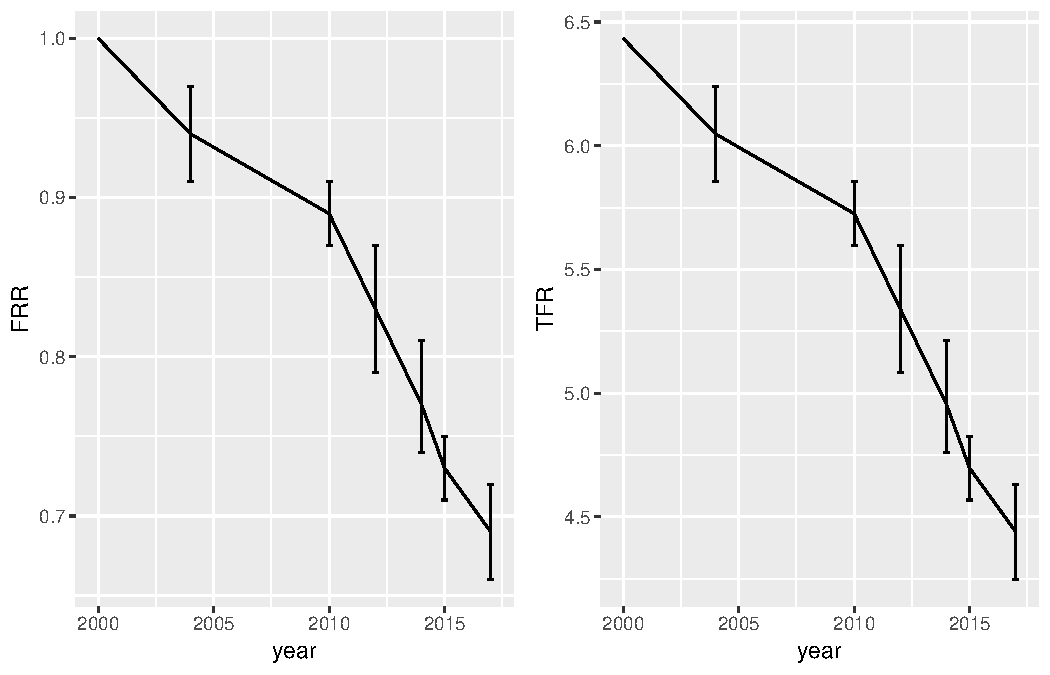
\includegraphics{test_vignette_files/figure-latex/unnamed-chunk-3-1.pdf}

Fertility by age group adjusted by time. Left hand plot - 15-19 is base
reference year. Right hand plot - multiplied by ASFR for 15-19
calculated from all surveys.

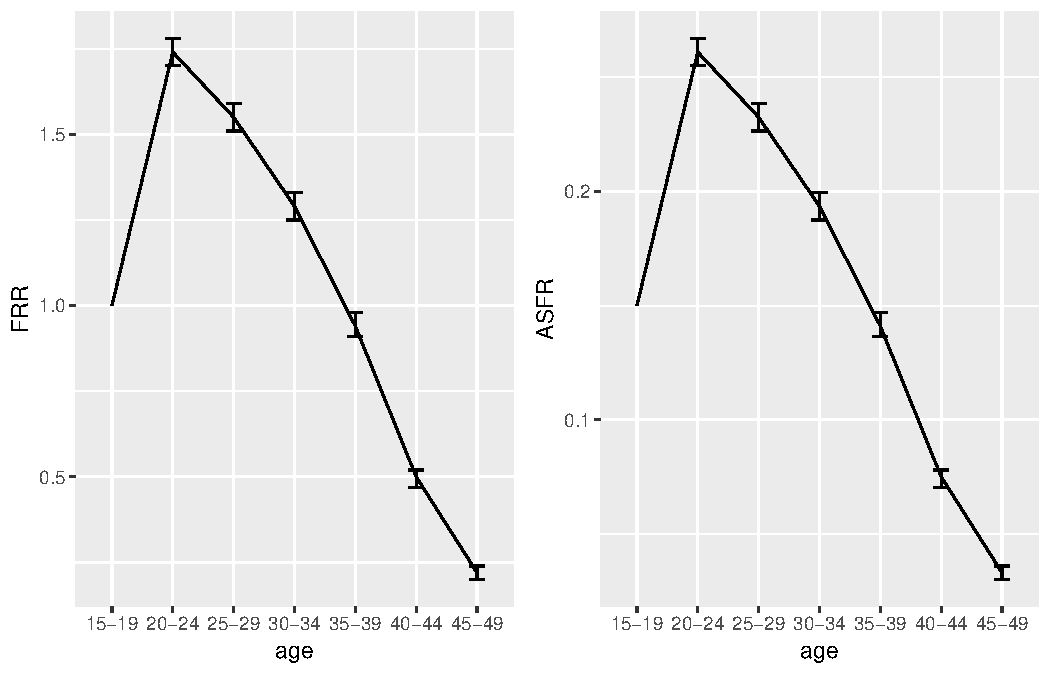
\includegraphics{test_vignette_files/figure-latex/unnamed-chunk-4-1.pdf}

With interaction between survey year and age group

\begin{Shaded}
\begin{Highlighting}[]

\NormalTok{m1 <-}\StringTok{ }\KeywordTok{glm}\NormalTok{(births }\OperatorTok{~}\StringTok{ }\NormalTok{survyear}\OperatorTok{*}\NormalTok{agegr, }\DataTypeTok{data=}\NormalTok{asfr_mod_data, }\DataTypeTok{family =} \KeywordTok{poisson}\NormalTok{(), }\DataTypeTok{offset=}\KeywordTok{log}\NormalTok{(pys))}
\end{Highlighting}
\end{Shaded}

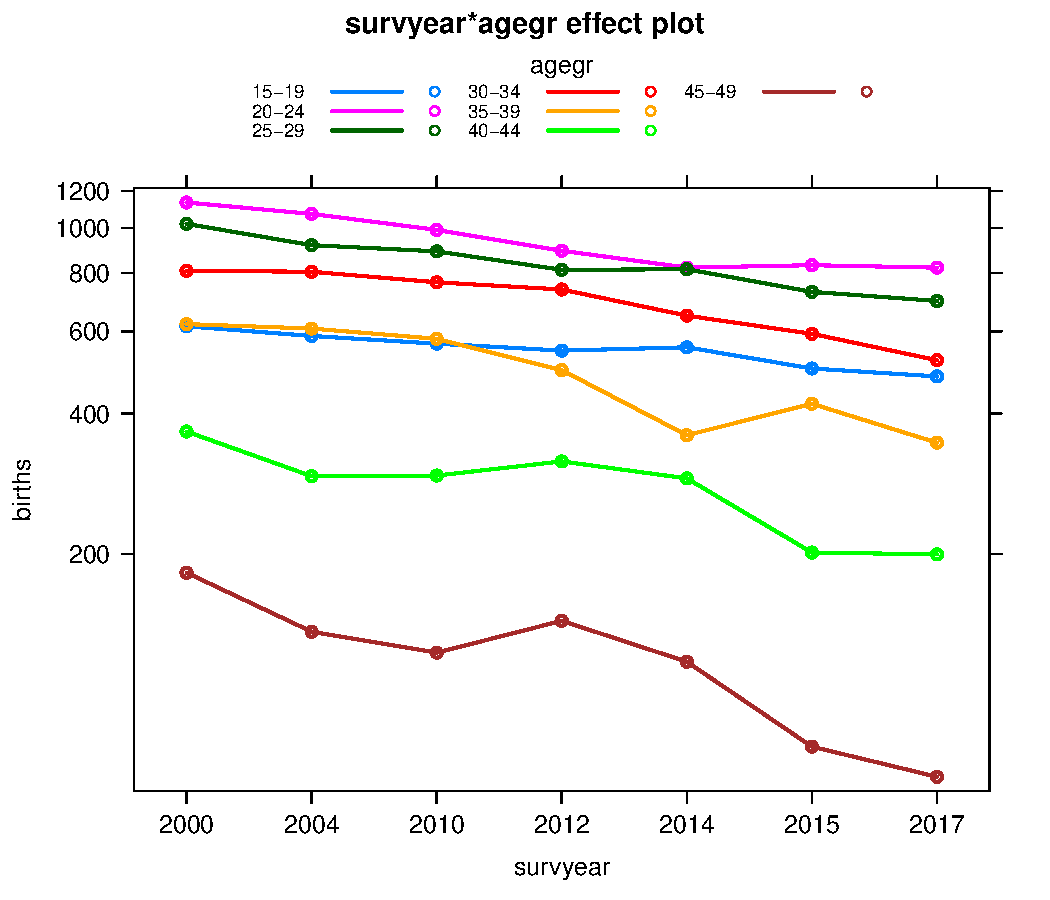
\includegraphics{test_vignette_files/figure-latex/unnamed-chunk-6-1.pdf}


\end{document}
